\chapter{Stato dell'Arte}
\section{Introduzione}
Negli ultimi anni, i sistemi informatici hanno assunto un ruolo sempre pi\`u centrale nelle attivit\`a umane.\\*
Inizialmente, il computer era considerato un semplice strumento di supporto alla matematica applicata, capace di svolgere calcoli particolarmente onerosi in un tempo relativamente breve. Con lo sviluppo delle tecnologie, i sistemi informatici sono ad oggi impiegati in un vasto insieme di domini applicativi, dall'elettromedicale al trasporto aereo, fino all'\emph{Internet of Things}.\\*
Quanto pi\`u si diffonde l'utilizzo dei sistemi informatici, tanto pi\`u peso assume un eventuale fallimento dei medesimi. La letteratura scientifica dimostra che la valutazione della \emph{dependability} di un sistema informatico \`e un problema chiave.\\*
Per \emph{dependability} si intende la capacit\`a che ha un sistema di fornire un servizio in modo corretto. \cite{depdef}\\*
Un \emph{fallimento} \`e una transizione compiuta da un sistema dall'erogazione di un servizio corretto verso l'erogazione di un servizio scorretto. La transizione contraria \`e detta \emph{restauro}.\\*
\begin{figure}[h]
	\centering
	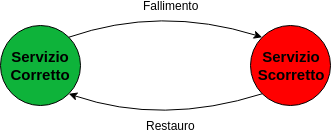
\includegraphics[width=0.7\linewidth]{img/FallimentoRestauro}
	\caption{Fallimento e restauro}
	\label{fig:fallimentorestauro}
\end{figure}\newpage
Effettuare misure sperimentali su un sistema informatico, o su un suo prototipo, \`e una valida opzione per valutarne la \emph{dependability}.\\*
Questa Tesi descrive l'attivit\`a di osservazione del prototipo di un sistema informatico impiegato nell'ambito del posizionamento ferrotramviario.
\subsection{Dependability}
La \emph{dependability} di un sistema \`e:
\begin{itemize}
	\item Misurata rispetto a un certo insieme di propriet\`a note come \emph{measures};
	\item Raggiunta attraverso l'utilizzo di specifiche tecniche, i \emph{means};
	\item Minacciata dai \emph{threats}, ossia da tutto ci\`o che porta il sistema ad erogare un servizio improprio.\\*
	Un sistema pu\`o fallire nel caso in cui questo non sia conforme alle specifiche, oppure perch\`e le specifiche non descrivono adeguatamente le sue funzioni.\\*
\end{itemize}
La \emph{dependability} di un sistema viene misurata rispetto alle seguenti propriet\`a:
\begin{itemize}
	\item \emph{Availability}: L'alternanza tra la fornitura di un servizio corretto e uno scorretto.
	$$
	A(t) = \begin{cases} 1 & \mbox{se il servizio fornito \`e corretto al tempo t} \\ 0 & \mbox{altrimenti} \end{cases}
	$$
	$\mathbb E[A(t)]:$ probabilit\`a che il servizio fornito sia corretto al tempo $t$
	\item \emph{Reliability}: Capacit\`a di fornire un servizio continuamente corretto in un certo intervallo di tempo.
	$$
	R(t):\mbox{probabilit\`a di fornire un servizio corretto nell'intervallo }[0,t]
	$$
	\item \emph{Safety}: Il tempo medio a un fallimento catastrofico.\\*\\*
	$S(t):$ probabilit\`a che non si verifichi alcun fallimento catastrofico nell'intervallo $[0,t]$\\*\\*
	La \emph{safety} \`e un' estensione del concetto di \emph{reliability}.\newpage
	Si definisce uno stato sicuro in cui il sistema:
	\begin{itemize}
		\item Fornisce il servizio corretto, oppure
		\item Non fornisce il servizio corretto, ma il fallimento non ha conseguenze catastrofiche sull'ambiente o sulle persone
	\end{itemize}
	Qualunque fallimento che induca il sistema a fornire un servizio scorretto con conseguenze catastrofiche, viene modellato come una transizione verso uno stato non sicuro.\\*
	\begin{figure}[h]
		\centering
		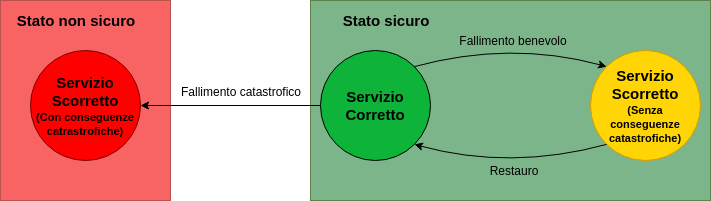
\includegraphics[width=0.7\linewidth]{img/safety}
		\caption{La \emph{safety} estende il concetto di \emph{reliability}}
		\label{fig:safety}
	\end{figure}
	\item \emph{Time to Failure}: Il tempo che intercorre fra l'ultimo restauro e il successivo fallimento.\\*
	Spesso \`e opportuno considerare il valore atteso di questa grandezza, il \emph{Mean Time to Failure} (MTTF)
	\item \emph{Maintainability}: Il tempo necessario a restaurare il sistema, dopo l'ultimo fallimento. Il valore atteso di questa misura prende il nome di \emph{Mean Time to Repair} (MTTR)
	\item \emph{Coverage}: Probabilit\`a che il sistema sia in grado di tollerare un guasto.
\end{itemize}
I \emph{threats} che minano la \emph{dependability} di un sistema sono i guasti, gli errori e i fallimenti.\\*
Un guasto \`e un qualunque evento interno al sistema in grado di causare un errore. Quando l'errore raggiunge l'interfaccia di servizio, ovvero altera il servizio fornito dal sistema, si parla di fallimento. In letteratura, si fa riferimento a questo rapporto di causalit\`a come \emph{fault error failure chain}, catena guasto errore fallimento.\\*
\begin{figure}[h]
	\centering
	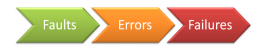
\includegraphics[width=0.7\linewidth]{img/gefpng}
	\caption{Catena guasto errore fallimento}
	\label{fig:gefpng}
\end{figure}\newpage
La \emph{dependability} di un sistema informatico \`e raggiunta attraverso l'uso di quattro tecniche:
\begin{itemize}
	\item \emph{Fault Prevention}: Previene l'insorgenza di guasti durante il ciclo di vita del sistema
	\item \emph{Fault Tolerance}: Rende il sistema in grado di fornire un servizio corretto anche in presenza di guasti
	\item \emph{Fault Removal}: Riduce il numero di guasti nel sistema
	\item \emph{Fault Forecasting}: Stima il numero di guasti presenti nel sistema, attualmente o in futuro
\end{itemize}
La \emph{dependability} \`e la propriet\`a che viene misurata durante il processo di \emph{validazione} di un sistema informatico.\\*
La validazione di un sistema informatico \`e un processo atto a determinare se il sistema \`e conforme alle sue specifiche funzionali.\\*
Il processo di validazione avviene durante tutte le fasi del ciclo di vita del sistema, anche prima che venga realizzato. Per questo motivo, il sistema viene opportunamente modellato al fine di condurre propriamente l'analisi.\\*
A discrezione della fase del ciclo di vita del sistema, si utilizzano differenti tecniche e modelli di validazione: \cite{librobonda}
\begin{itemize}
	\item Specifica: la validazione \`e basata sull'utilizzo di tecniche combinatorie che mirano a determinare le condizioni di fallimento di un sistema in funzione del fallimento dei suoi sottocomponenti, considerati indipendenti;
	\item \emph{Design}: in questa fase si usano tecniche analitiche, come ad esempio le Catene di Markov, che permettono di rilassare le assunzioni di indipendenza tipiche dei modelli combinatori;
	\item Implementazione: con il procedere della fase di implementazione, il sistema prende forma e pu\`o essere interessante osservarne direttamente il comportamento ed effettuare misure sperimentali;
	\item Fase operativa: il sistema \`e impiegato sul campo e possono quindi essere utilizzate tutte le tecniche disponibili per l'analisi.
\end{itemize}


\section{Robaccia}
\`E possibile schematizzare un sistema ferroviario, o ferrotramviario, come un insieme di vetture vincolate a muoversi lungo una traccia fissata.\\*
Questa schematizzazione \`e, in grossolana approssimazione, valida per qualsiasi sistema ferroviario o ferrotramviario, a prescindere dal numero di veicoli transitanti o dall'estensione geografica. Ci\'o che invece differenzia un sistema ferroviario da un sistema ferrotramviario sono:
\begin{itemize}
		\item Le caratteristiche fisiche del veicolo transitante, come lunghezza e massa;
		\item Le caratteristiche geografiche dell'ambiente operativo;
		\item Gli scopi del trasporto.
\end{itemize}
In generale, nel trasporto ferroviario si utilizzano veicoli pesanti atti a trasportare persone o merci su lunghe percorrenze, pertanto \`e comune che l'ambiente operativo di un sistema ferroviario sia prevalentemente extra urbano.\\*
Nel trasporto ferrotramviario, di contro, si utilizzano veicoli leggeri per offrire un'alternativa al cittadino all'utilizzo di mezzi privati durante i suoi spostamenti all'interno di un'area metropolitana. Quest'ultima caratteristica implica che l'ambiente operativo di un sistema ferrotramviario sia radicalmente diverso dall'ambiente operativo di un sistema ferroviario. Le vetture si muovono lungo traccie installate su strade urbane, e di conseguenza il traffico ferrotramviario condivide l'ambiente con il traffico cittadino, come mostrato in figura \ref{fig:tramschema}.\\*
\begin{figure}[h]
		\centering
		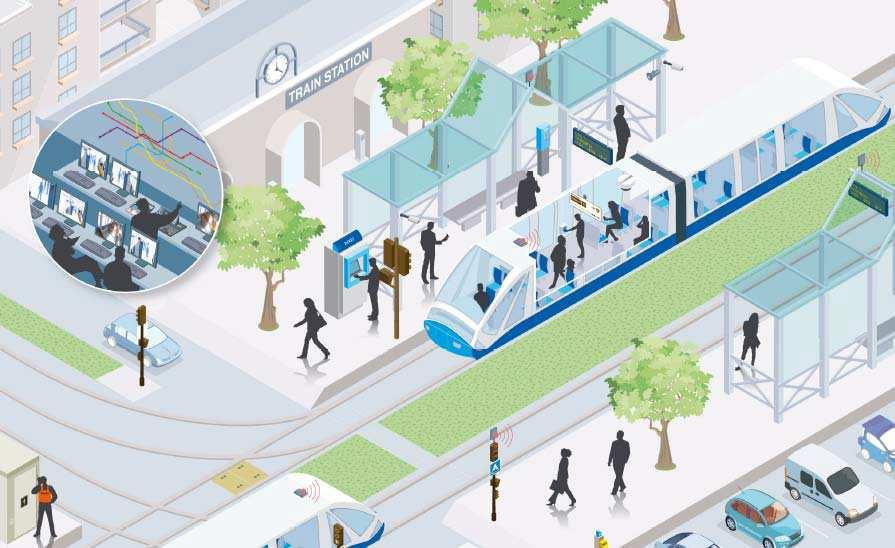
\includegraphics[width=0.7\linewidth]{img/twschema}
		\caption{Schema di un tipico scenario ferrotramviario}
		\label{fig:tramschema}
\end{figure}
\section{Il problema del posizionamento}
Per posizionamento ferroviario si intende la valutazione della posizione di un treno all'interno di una traccia ferroviaria. Tale posizione viene espressa come progressiva chilometrica rispetto a una posizione nota, come ad esempio l'origine della linea. \cite{trainpositioning}\\*
\subsubsection{Odierne Tecniche di Posizionamento}
Gli odierni sistemi di posizionamento si basano principalmente sull'utilizzo di strumenti installati a terra, chiamati \emph{beacon}, o \emph{balise} in gergo ferroviario, i quali hanno lo scopo di rilevare il passaggio di un treno.\cite{tecnicheodierne}
Esiste uno standard a livello europeo al quale gli odierni sistemi di posizionamento si devono uniformare, l' \emph{European Train Control System} (ETCS).\\*
Nel corso della storia, ogni paese europeo ha sviluppato autonomamente le proprie infrastrutture ferroviarie e relative regole operative. Tuttavia, ad oggi i treni possono attraversare le frontiere, pertanto \`e necessario sviluppare un sistema ferroviario standard che rispetti una comune normativa operazionale europea. Tale sistema prende il nome di \emph{European Rail Traffic Management System} (ERTMS) \cite{ertms}, ed ETCS \`e il sottosistema di ERTMS dedicato al posizionamento delle vetture.\\*
Come standard, ETCS definisce specifici livelli di \emph{compliance} che possiede un sistema di posizionamento rispetto ad ETCS, ed essi vanno dal livello \texttt{ETCS-0} al livello \texttt{ETCS-3}. \cite{svolta}
\\*
L'obiettivo \`e quello di sviluppare progressivamente un sistema di posizionamento completamente autonomo (\texttt{ETCS-3}), partendo da un sistema interamente \emph{non-compliant} con ETCS (\texttt{ETCS-0}).
\\*
Allo stato attuale, quasi tutti i sistemi di posizionamento sono \texttt{ETCS-2}. Nei livelli \texttt{ETCS-1} e \texttt{ETCS-2}, le traccie vengono suddivise in blocchi, e all'entrata di ciascun blocco viene posizionato un \emph{beacon} in grado di rilevare la presenza di un treno.\\*
L'autorizzazione all'ingresso in un blocco viene rilasciata se nessun altro treno sta occupando il blocco al quale si vuole accedere, mentre un sistema di \emph{odometria} installato a bordo, posiziona il treno rispetto all'ultimo \emph{beacon} incontrato.\\*
Nel livello \texttt{ETCS-3}, non sono richiesti segnali provenienti dalla linea: un treno deve essere in grado di posizonarsi autonomamente. \cite{etcs3}\\*
In sintesi, i livelli ETCS possono essere descritti come segue:
\begin{itemize}
	\item \texttt{ETCS-0}: Sistema non conforme a ETCS;
	\item \texttt{ETCS-1}: Utilizzo di apparati di posizionamento installati a terra, autorizzazione a procedere segnalata al macchinista attraverso indicazioni semaforiche;
	\item \texttt{ETCS-2}: Come \texttt{ETCS-1}, ma l'autorizzazione a procedere \`e gestita da un sistema automatico di scambio, denominato sistema di \emph{interlocking};\cite{interlocking}
	\item \texttt{ETCS-3}: Posizionamento autonomo, nessun utilizzo di apparati a terra.
\end{itemize}
\begin{figure}[h]
	\centering
	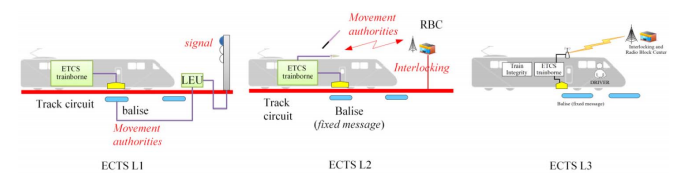
\includegraphics[width=\linewidth]{img/etcs123.png}
	\caption{Livelli \texttt{ETCS}}
	\label{fig:etcs123}
\end{figure}
Il livello \texttt{ETCS-2} prevede che l'autorizzazione a procedere venga gestita dal sistema di \emph{interlocking} e non dal solo operatore umano notificato mediante indicazioni semaforiche.\\*
La funzionalit\`a offerta del sistema di \emph{interlocking} viene pertanto considerata \emph{safety-critical}, in quanto un suo fallimento pu\`o portare a conseguenze anche catastrofiche.\cite{marocchini}\\*
ETCS adotta un approccio incrementale alla realizzazione di sistemi di posizionamento autonomi. Un sistema di posizionamento \texttt{ETCS-3} deve continuare a interagire con il sistema di \emph{interlocking}, quindi deve essere considerato a sua volta un sistema \emph{safety-critical}.\\*
L'implementazione hardware e software di un sistema \texttt{ETCS-3} viene dunque vincolata da standard generici per sistemi \emph{safety-critical} \cite{MISRA} \cite{sil}, e da standard specifici del dominio ferroviario \cite{50128}.\\*
ERTMS/ETCS \`e pensato per sistemi ferroviari, mentre nel dominio ferrotramviario vige la regola della \emph{marcia a vista}. Il rispetto di ETCS non \`e obbligatorio in detto contesto, tuttavia le tecniche di posizionamento ivi utilizzate rispettano spesso le linee guida imposte da ETCS. 
\section{Verso ETCS-3}
Gli attuali sistemi di posizionamento richiedono un minimo intervento di computer installati a bordo e una grande quantit\`a di apparati installati a terra. Gli apparati di terra sono costosi e hanno un impatto ambientale non trascurabile, pertanto \`e necessario iniziare a pianificare una migrazione verso sistemi \texttt{ETCS-3}.\cite{market}\\*
Il sistema oggetto della Tesi \`e un sottosistema di posizionamento conforme alla filosofia \texttt{ETCS-3}.\\*
Nell'ottica di voler realizzare un sistema di posizionamento autonomo, il treno viene modellato come un \emph{Cyber-Physical System} (CPS).\\*
Un CPS \`e un sistema che consiste di un computer (sottosistema \emph{cyber}) e un oggetto da esso controllato (sottosistema \emph{physical}).
Il sottosistema \emph{cyber} \`e essenzialmente un elaboratore che opera in un tempo discreto, dispone di processore, memoria, e di interfacce I/O che abilitano l'interazione del CPS con eventuali operatori umani.\\*Il sottosistema \emph{physical} consiste di un sistema governato dalle leggi della fisica che opera in un tempo continuo.
\cite{cps}\cite{cecca}\\*
Nella fattispecie, l'oggetto controllato \`e il treno, mentre l'elemento \emph{cyber} \`e costituito da un \emph{sistema di sistemi} composto da un'unit\`a in grado di campionare e processare un certo insieme di misure, e da un'unit\`a in grado di controllare il movimento del treno. Quest'ultima unit\`a prende il nome di \emph{On Board Control Unit} (OBCU), ed \`e il computer di bordo nominale che ogni treno deve possedere in accordo a ERTMS/ETCS.\\*
Lo scopo della Tesi \`e quello di mostrare i risultati sperimentali delle campagne di analisi condotte sul sottosistema \emph{cyber} del CPS descritto.\\*
Tale sottosistema ha lo scopo di stimare la posizione di un treno attraverso l'uso combinato di un insieme di sensori installati a bordo.\\*
I valori campionati dai sensori dovranno essere integrati al fine di ottenere una stima sicura e affidabile della posizione del treno. Tale integrazione viene realizzata grazie all'utilizzo di un algoritmo noto come \emph{Sensor Fusion Algorithm} (SFA). \cite{sfarailway}\\*
Nello sviluppo di un sistema di posizionamento \emph{safety-critical}, \`e fondamentale poter garantire che l'errore commesso dal sistema non superi una determinata soglia.\\*
Le analisi condotte si prefiggono lo scopo di poter osservare sperimentalmente una situazione in cui l'errore commesso non superi una determinata soglia definita come accettabile.